\documentclass[letterpaper,twocolumn,10pt]{article}

\usepackage{tikz}
\usepackage{amsmath}
\usepackage{graphicx}
\usepackage{float}
\usepackage{lipsum}
\usepackage{sidecap}
\usepackage{hyperref}
\usepackage{xcolor}

\usepackage{titling}

%\usepackage[left=0.5in,right=0.5in, bottom=0.5in]{geometry}
\setlength{\droptitle}{-0.5in}
\usepackage[margin=0.5in]{geometry}



%-------------------------------------------------------------------------------
\begin{document}
% -------------------------------------------------------------------------------

\date{} % avoid printing of date

\title{Serial-Optimising Chessboard-Pattern Stenciling}

\author{
  {\rm Jan Fecht}\\
  University of Bristol}

\maketitle


% -------------------------------------------------------------------------------
\section*{Introduction}
% -------------------------------------------------------------------------------
The program to be optimised consists of a simple stencil applied on a chessboard-pattern image.
The user can specify the width $nx$ and the height $ny$ of the image and furthermore
the number of times $k$ that the stencil is applied. All of these parameters are passed on the command line to the program, except for $k$ which is passed as $k/2$ (niters) instead.

For comparing and evaluating the effect of
a particular optimisation, the final version of the code was benchmarked
and compared to the final version without the optimisation.

Measured times were determined by taking the average of 100 runs
on the University's \textit{Blue Crystal 4} supercomputer (bc4). The times for
the original version were taken from the official repository
\footnote{\url{https://github.com/UoB-HPC/intro-hpc-stencil/}} instead as running it 100 times would have been infeasible.

The speedup of the final version can be seen in Table~\ref{tab:final}.

\vspace{0.15in}

\textbf{Disclaimer} The optimisations applied may have neither been introduced
in the order nor grouped together as they are described in this report. Rather, the 
whole optimisation process was iterative because new ideas and adaptions to new
circumstances were necessary. Therefore most comparisons were conducted by removing
a whole set of similar optimisations made and comparing it to the version with them.

\begin{table}[ht]
	\caption{Final compared to the original version ($k=200$).}
	\begin{tabular}{c c c c}
		 image size & original & final & speedup \\
		 \hline
		1024 x 1024 & 5.908341s   & 0.01703819s & 346.77 \\
		4096 x 4096 & 130.196475s & 0.02655836s & 4902.28\\
		8000 x 8000 & 561.118133s & 0.04257847s & 13178.45\\
	\end{tabular}
	\label{tab:final}
\end{table}

% -------------------------------------------------------------------------------
\section*{Algorithm}
% -------------------------------------------------------------------------------
The chessboard pattern contains a high degree of symmetry and by applying the stencil code
to all points the original code performs plenty of redundant computations.
The number of floating point operations lies in $\Theta(nx * ny * k)$
as the number of points to be stenciled is $nx * ny$.
To reduce this number drastically, one can stencil only small parts of the image and apply
these precomputed parts to the whole image by copying and possibly mirroring or inverting them.
The specific parts that need to be precomputed can be seen
in Figure~\ref{fig:board} as the opaque fields. The center part in \textcolor{red}{red} cannot
be applied to the whole image but only to the center in transparent red.
The reason for this lies in the way the borders are stenciled in the original version. It assumes
that there is an invisible black border around the field. This leads to a slightly darker border
which affects all pixels in a range of $k$ around the border. This is marked as the
\textcolor{green}{green}, \textcolor{blue}{blue} and \textcolor{yellow}{yellow} parts in Figure~\ref{fig:board}.

\begin{figure}[t]
	\begin{center}
	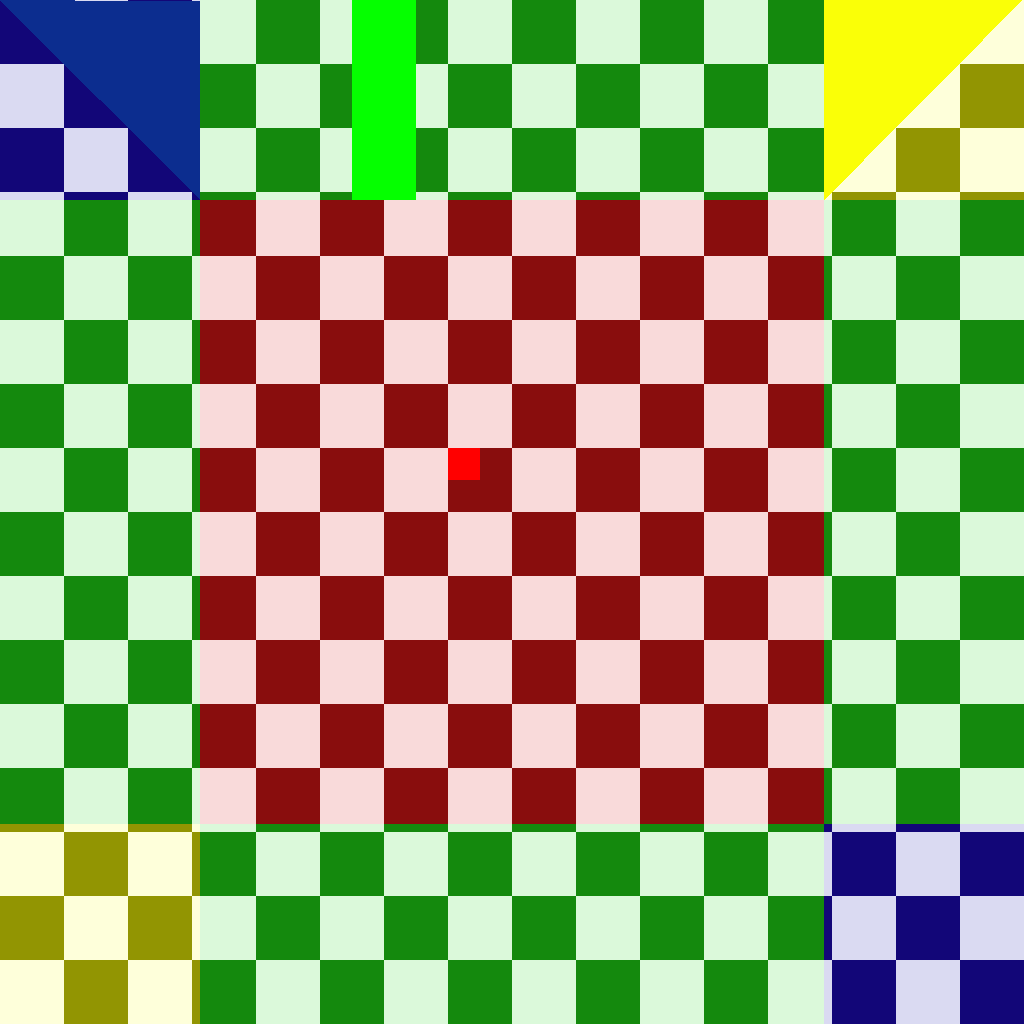
\includegraphics[width=150pt]{res/stencil_colored_with_prec}
	\caption{Colored 1024 x 1024 pattern assumming $k = 200$. Areas that need to be precomputed in opaque.}
	\label{fig:board}
	\end{center}
\end{figure}

The \textcolor{blue}{blue} corners can only be reused for the \textcolor{yellow}{yellow} corners
if they share the same colored (black or white) tile in the most outer part of the edge. This is only the
case if ($nx + ny) \equiv_{128} 0$

If either $nx \not\equiv_{64} 0$ or $ny \not\equiv_{64}0$, the right border or lower border, respectively, need to be computed additionally.
Furthermore all corners need to be computed seperatly. For all corners except the top-left one,
we even need to compute the whole field, because we loose the symmetry of the diagonal.  
This leads to the number of tiles to be stenciled in Table~\ref{tab:numstencil}. Note that
in the last case of the table, only the worst case is specified, as the optimised program
tries to find further symmetries (e.g. between right and lower border).

Because the number of tiles to be stenciled lies in $\Theta(k^2)$, the number of floating-point
operations lies in $\Theta(k^3)$ and is therefore asymptotically independent of the dimensions of the image. That also explains the small differences of times in Table~\ref{tab:prec} with precomputation compared to the bigger differences without.
If this optimisation does not decrease the number of tiles to be stenciled, the program falls back to stenciling the whole field.

\begin{table}[ht]
	\caption{Number of tiles to be stenciled}
	\begin{tabular}{c c}
		variables & number of tiles\\
		\hline
		$\scriptstyle nx,ny \equiv_{64}0,(nx+ny) \equiv_{128}0$ & $ \frac{k(k+1)}{2} + 64k + 32^{2}$\\
		$\scriptstyle nx,ny \equiv_{64}0,(nx+ny) \not\equiv_{128}0$ & $ k(k+1) + 64k + 32^{2}$\\
		$\scriptstyle nx \not\equiv_{64}0 \lor \scriptstyle ny \not\equiv_{64}0$ & $ 3k^{2} + \frac{k(k+1)}{2} + 3 * 64k + 32^{2}$\\
	\end{tabular}
	\label{tab:numstencil}
\end{table}


\begin{table}[ht]
	\caption{Final version with and without precomputation ($k=200$).}
	\begin{tabular}{c c c c}
		image size    & w. prec.   & w.o. pre.    & speedup   \\
		 \hline
		 1024 x 1024 & 0.01703819s & 0.1301483s   & 7.6386    \\
		 4096 x 4096 & 0.02655836s & 3.53007045s  & 132.9174  \\
		 8000 x 8000 & 0.04257847s & 14.22400545s & 334.0657  \\
	\end{tabular}
	\label{tab:prec}
\end{table}


\section*{Access Pattern}
Although the Algorithm

\section*{Vectorisation}
%- Alignment
%- \_\_builtin\_assume\_aligned
%- speedups
%- replace memcpy with for loops
The processor found on the bc4 is the \textit{Intel Xeon E5-2680 v4} introduced in 2016.
According to the official intel spreadsheet\footnote{\url{https://ark.intel.com/content/www/us/en/ark/products/91754/intel-xeon-processor-e5-2680-v4-35m-cache-2-40-ghz.html}},
it supports the \textit{AVX2} instruction extension, which allows vector operations on up to 256 bits.

\section*{Other Improvements}
- compiler flags
- failed attempts

\section*{Further possible Improvements}

% -------------------------------------------------------------------------------
\section*{Conclusion}
% -------------------------------------------------------------------------------


\bibliographystyle{plain}
\bibliography{lit}

\end{document}
